\documentclass[10pt,a4paper,titlepage]{article}
\usepackage[utf8]{inputenc}
\usepackage[T1]{fontenc}
\usepackage[english]{babel}
\usepackage{amsmath}
\usepackage{amsfonts}
\usepackage{amssymb}
\usepackage{graphicx}
\usepackage{fullpage}
\usepackage{float}
\usepackage[detect-all]{siunitx} 
\usepackage{xcolor}

\usepackage{csquotes}

\usepackage{listings}

\usepackage[pdftex]{hyperref}
\hypersetup{            
	colorlinks=true,      
	pdfpagemode=UseNone,     
	linkcolor = black,
	filecolor = darkgreen,
	urlcolor = blue,
	citecolor = blue,
	bookmarksopen,        
	bookmarksnumbered,    
	bookmarksopenlevel=2,
	pdfmenubar=true,
	pdfwindowui=true
}

\usepackage[backend=biber,style=ieee]{biblatex}
\addbibresource{references.bib}


\author{
Werner Simbürger\\ \href{mailto:werner.simbuerger@hppi.de}{werner.simbuerger@hppi.de}
\and
Arved Enders-Seidlitz \\ \href{mailto:arved.enders-seidlitz@ikz-berlin.de}{arved.enders-seidlitz@ikz-berlin.de}}


\title{pyelmer Example: 3D Electrostatic Capacitance}



%%%%%%%%%%%%%%%%%%%%%%%%%%%%%%%%%%%%%%%
%% Macros
%%%%%%%%%%%%%%%%%%%%%%%%%%%%%%%%%%%%%%%
\newcommand{\fig}[1]{Fig.~\ref{#1}}
\newcommand{\tab}[1]{Tab.~\ref{#1}}
\newcommand{\eqn}[1]{Eqn.~\ref{#1}}
\newcommand{\sect}[1]{Sect.~\ref{#1}}
\newcommand{\note}[1]{Note~\ref{#1}}
\newcommand{\up}[1]{\textup{#1}}


\definecolor{codegreen}{rgb}{0,0.6,0}
\definecolor{codegray}{rgb}{0.5,0.5,0.5}
\definecolor{codepurple}{rgb}{0.58,0,0.82}
\definecolor{backcolour}{rgb}{0.95,0.95,0.92}



\begin{document}
	\maketitle
	\tableofcontents
\clearpage
\section{Problem Description}

The 3D electrostatic capacitance including fringing between top metal and bottom metal (\fig{3835848427}) shall be calculated with Elmer FEM \cite{ElmerFEM}, Gmsh \cite{Gmsh} and Python \cite{WinPython} including the pyelmer \cite{pyelmer} package. ParaView \cite{ParaView} is used to review the calculated FEM results, such as vector fields.


\begin{figure}[H]
  \begin{center}
     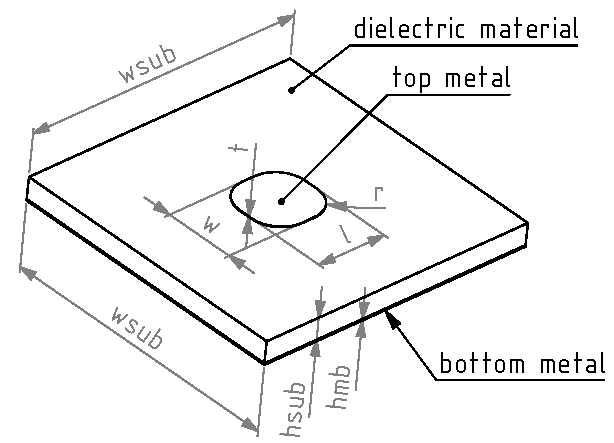
\includegraphics[width=!, height=5cm, angle=0]{./fig/example_01.pdf}
     \caption{3D electrostatics capacitance}
     \label{3835848427}
  \end{center}
\end{figure}

\noindent
The top metal has a width $w$, length $l$ and metal layer thickness $t$. The corners of the top metal patch have a fillet $r$.
The dielectric material layer has a relative permittivity $\epsilon_r$, thickness $hsub$, width and length $wsub$.
The bottom metal layer has a layer thickness $hmb$. The entire stack is surrounded by air.

\section{Solution}

\subsection{Analytical Calculation}

To verify the Elmer FEM computation of the capacitance, we can use a special geometrical case $w = l$, $r \rightarrow w/2 = l/2$ and $t=hmb \ll hsub$, which results in a circular microstrip disk, as shown in \fig{3836149517} and presented in the paper \cite{1130017}.

\begin{figure}[H]
	\begin{center}
		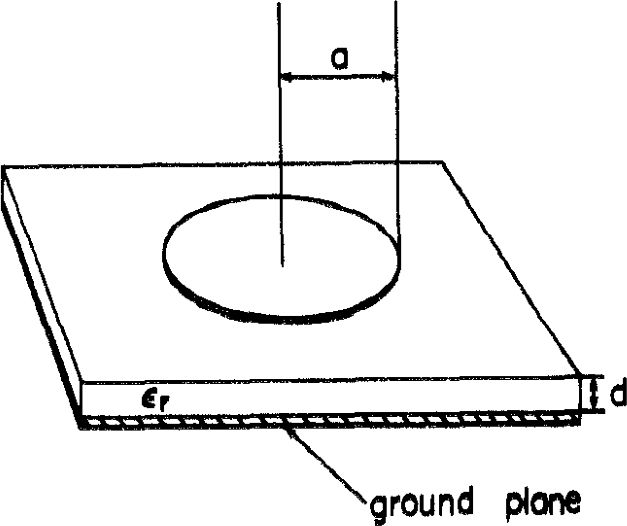
\includegraphics[width=!, height=5cm, angle=0]{./fig/disk.jpg}
		\caption{Effects of fringing fields on the capacitance of a circular microstrip disk \cite{1130017}}
		\label{3836149517}
	\end{center}
\end{figure}
\noindent
The authors of the paper \cite{1130017} present a quite accurate approximation formula for the capacitance within the parameter range of $\epsilon_r = 1 \text{ to } 8.5$ and $d/a = 0.1 \text{ to } 0.5$ as follows:
\begin{equation}
C \approx \frac{a^2 \pi \epsilon_r \epsilon_0}{d} \left\lbrace  1 + \frac{2d}{\pi \epsilon_r a}   \left[  \ln \left(\frac{a}{2 d}\right) + (1.41 \epsilon_r + 1.77) + \frac{d}{a} (0.268 \epsilon_r + 1.65) \right] \right\rbrace \label{3835945702}	
\end{equation}

\noindent
where the dielectric permittivity of vacuum $\epsilon_0 = \SI{8.854e-12}{\coulomb\per\volt\per\meter}$.

\subsection{Elmer FEM Calculation}


Prerequisite is the installation of the following software packages\footnote{available for Windows, Linux, Mac. References shown mainly for Windows.}:
\begin{enumerate}
	\item Elmer FEM solver \cite{ElmerFEM}
	\item Python $\geq$ 3.7 \cite{WinPython} including the pyelmer package \cite{pyelmer}
	\item ParaView \cite{ParaView} (optional)
\end{enumerate}

\noindent
The installation of the Elmer FEM solver and the Python/pyelmer package is mandatory. Gmsh is part of the Python pyelmer package. However, for debugging purposes the independent Gmsh software can be installed in parallel.
ParaView is optional, but it is extremely helpful to review the Elmer FEM calculated results (\verb|*.vtu|), such as vector fields.

Copy the files \verb|3d_electrostatic_capacitance.py|, \verb|my_simulations.yml|, \verb|my_solvers.yml| and \verb|my_materials.yml| in a local folder and run \verb|3d_electrostatic_capacitance.py|.

The entire geometry definition, mesh creation, Elmer FEM calculation and results evaluation process is executed by a single Python/pyelmer top level script \verb|3d_electrostatic_capacitance.py|, which is listed in \sect{3835864466}.




\section{Test Case and Results}

\subsection{Test Case Parameter}

The structure shown in \fig{3835848427} is simulated with the following parameters:

\begin{table}[H]
\centering
\begin{tabular}{lrll}
\bf Parameter & \bf Value & \bf Unit  & \bf Description \\
$w$ & 6 & \si{\milli\meter}	& top metal patch width \\
$l$ & 6 & \si{\milli\meter}	& top metal patch length \\
$t$ & 0.035 & \si{\milli\meter}	& top metal layer thickness \\
$r$ & 2.95 & \si{\milli\meter}	& top metal patch corner radius (fillet) \\
$hsub$ & 1.524 & \si{\milli\meter}	& dielectric material layer thickness \\
$wsub$ & 24 & \si{\milli\meter}	& dielectric material layer width\\
$\epsilon_r$ & 3.55 & 	& dielectric material layer relative permittivity (Rogers RO4003C material \cite{RO4003C})\\
$hmb$ & 0.1 & \si{\milli\meter}	& bottom metal layer thickness \\
\end{tabular}
\caption{Test case parameter}
\end{table}

\subsection{Capacitance Calculation Results}

\begin{table}[H]
\centering
\begin{tabular}{ll}
Analytical solution (\eqn{3835945702}) & $C=\SI{1.012}{\pico\farad}$	\\
Elmer FEM computation & $C=\SI{1.062}{\pico\farad}$ \\
\end{tabular}
\caption{Analytical solution and Elmer FEM computation result of the capacitance}
\end{table}

\noindent
The Elmer FEM computation result listing, CPU-time of the Elmer solver in [second], excluding meshing:
\begin{verbatim}
Errors: []
Warnings: []
Statistics: {'CPU-time': 86.6, 'real-time': 86.6}
Relative Change: 5.10E-12
##############################################
w: 6E-3
l: 6E-3
r: 2.95E-3
Capacitance: 1.062E-12
##############################################
\end{verbatim}

\noindent
The agreement of the Elmer FEM computation result with the approximation formula \eqn{3835945702} is very good. However, it is very important to have small mesh size in the regions of high field gradients (\fig{3835951521}). Otherwise the Elmer FEM computation result may be significant wrong despite fast FEM algorithm convergence.

\begin{figure}[H]
	\begin{center}
		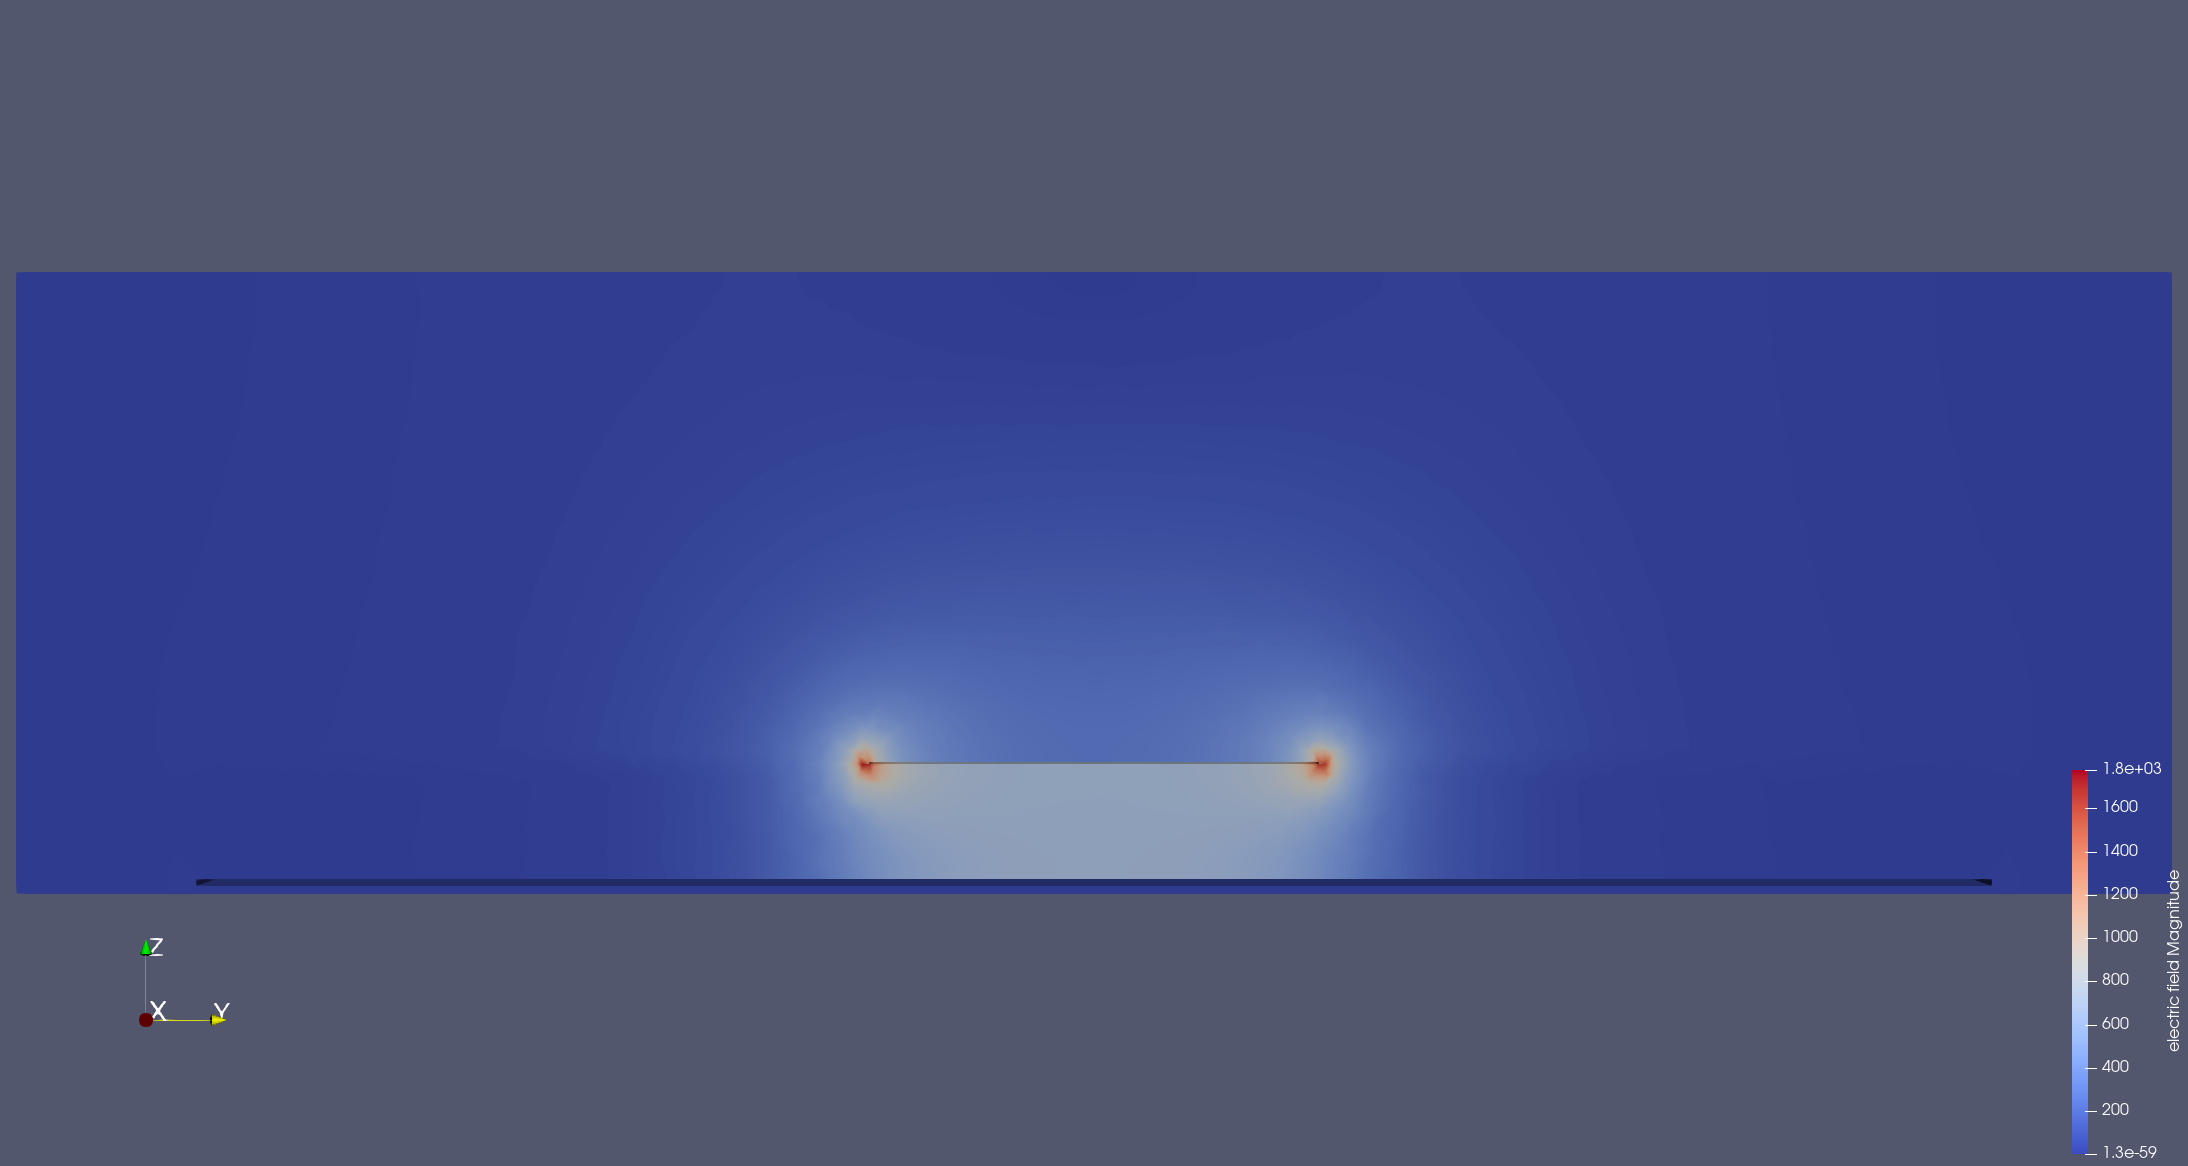
\includegraphics[width=!, height=6cm, angle=0]{./fig/e_field.png}
		\caption{Calculated electric field magnitude (cross section of \fig{3835947430})}
		\label{3835951521}
	\end{center}
\end{figure}


\subsection{Discussion of the Elmer FEM Solution and Boundary Conditions}

\begin{enumerate}
	\item The surrounding air of the structure is modeled by a proper air box, as shown in \fig{3835947430}. The size of the air box is calculated in line 123 and 124 (see \sect{3835864466}). The top height of the air box is designed properly in order to cover the fringing field in the air.
	
	\begin{figure}[H]
		\begin{center}
			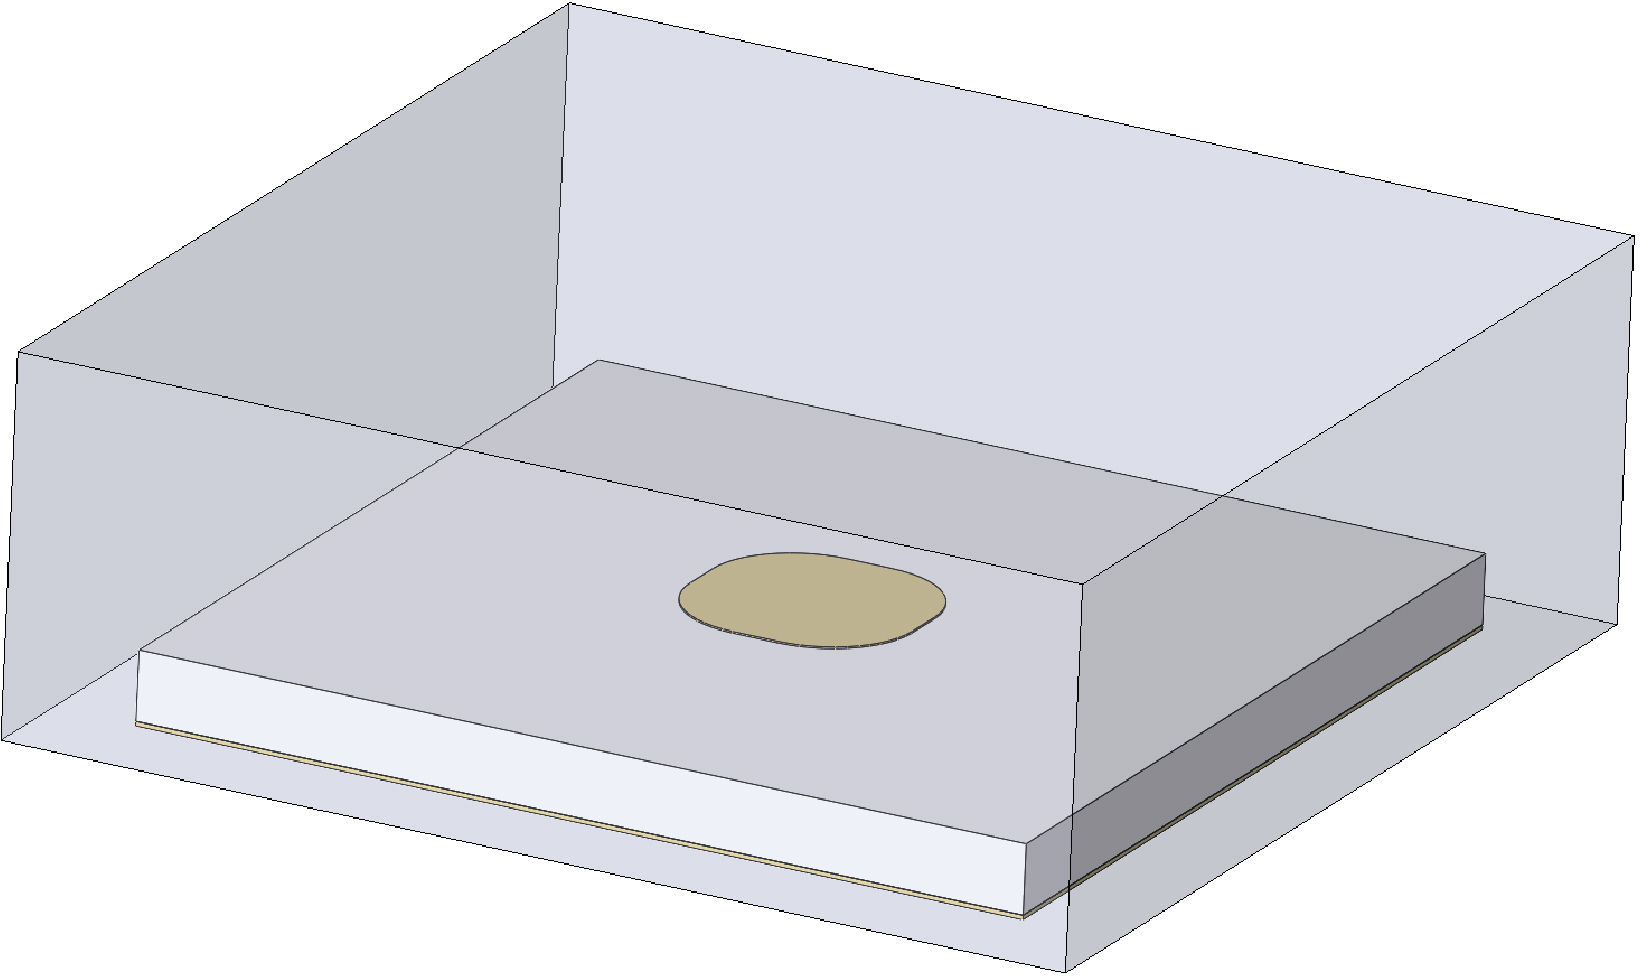
\includegraphics[width=!, height=6cm, angle=0]{./fig/example_01.JPG}
			\caption{3D model including air box}
			\label{3835947430}
		\end{center}
	\end{figure}
	
	\item The top metal and bottom metal layer are considered as perfect conductor. Therefore, these two bodies are not meshed in order to keep the required FEM meshing time and FEM computation time as low as possible. As a consequence, the structure consists of only two bodies (see line 128) which are required to be meshed:
	\begin{enumerate}
		\item dielectric material layer
		\item air box
	\end{enumerate}

\item To calculate the electrostatic capacitance between bottom metal and top metal, all surfaces need to be assigned to a potential value. All bottom metal body surfaces (there are 6 surfaces) are assigned to a potential of \SI{0}{\volt}. All top metal body surfaces (there are 10, because of the corner radius) are assigned to a potential of \SI{1}{\volt}. Further, it is very important to assign the correct value of the potential difference (line 269). Otherwise a wrong capacitance value will be calculated.

\begin{figure}[H]
\begin{center}
	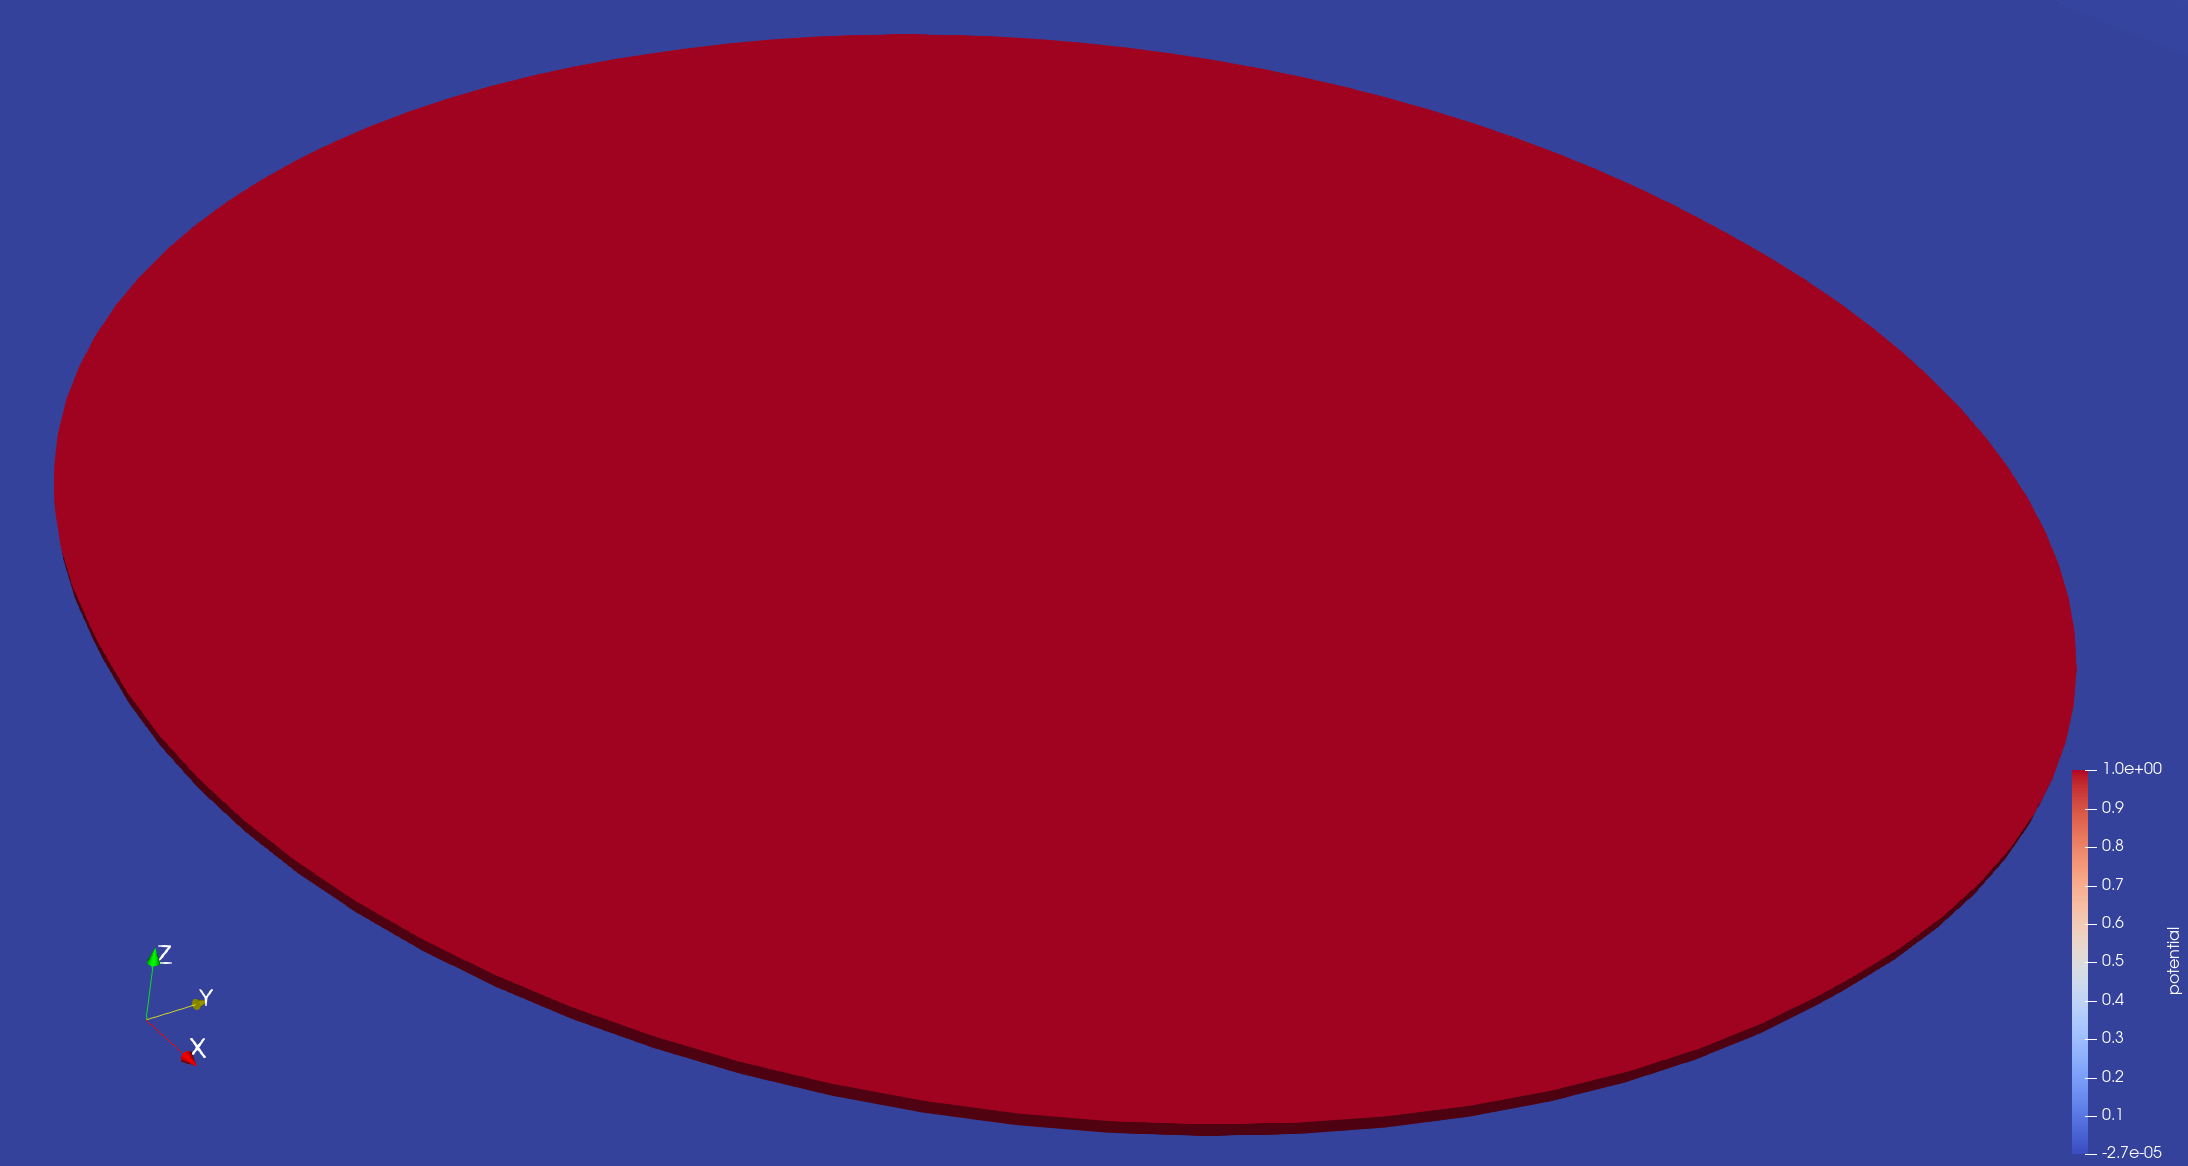
\includegraphics[width=!, height=6cm, angle=0]{./fig/potential.png}
	\caption{Potential distribution (top metal zoom view)}
	\label{3835951432}
\end{center}
\end{figure}


\item The correct assignment of physical bodies and boundary conditions are essential. The assignment of physical groups is semi-automated in this example, e.g. line 193, 194. The entity numbers of surfaces and physical group assignment is done automatically (e.g. line 205, 206). The general step approach of 3D modeling using pyelmer and Gmsh can be summarized as follows: 

\begin{enumerate}
	\item 3D modeling of the structure using Gmsh API functions
	\item Assign (only one time!) physical groups of required bodies
	\item Assign boundaries using the style \verb|id_for_elmer = add_physical_group(...)|. This can be done with automatic extraction using functions such as \verb|getMyEntitiesInBoundingBox| or by manual assignment, e.g. \verb|ph_sub, ph_ab| at line 193, 194.
	\item Meshing using Gmsh API functions
	\item Use Gmsh GUI to check if the assignment (step 2 above) is correct: press Ctrl+V, afterwards click through the physical groups
	\item For the definition of bodies use the \verb|id_for_elmer| from step 2 above
\end{enumerate}



\item Meshing notes:
The set up of the mesh including optimization is done using the Gmsh application programming interface (API) \cite{GmshAPI}. 
The geometric meshing parameters could be further optimized. However, it works well at this point of time, but the FEM computation time and meshing time could be further reduced by an optimized mesh.

\end{enumerate}


\section{Source File Listings}

\subsection{Python (pyelmer) Script}\label{3835864466}

The following Python script is based on pyelmer \cite{pyelmer} and is used to set up and run the Elmer FEM simulation from Python including model geometric parameter definition, meshing, definition of boundary conditions, Elmer FEM simulation and extraction of results. 

\clearpage

% Define a custom style
\lstdefinestyle{myStyle}{
backgroundcolor=\color{white},   
keywordstyle=\bfseries\color{blue},
commentstyle=\itshape\color{codegreen},
identifierstyle=\color{black},
stringstyle=\color{codepurple},
basicstyle=\ttfamily\footnotesize,
breakatwhitespace=false,         
breaklines=true,                 
keepspaces=true,                 
numbers=left,       
numbersep=5pt,                  
showspaces=false,                
showstringspaces=false,
showtabs=false,                  
tabsize=2,
}


\lstset{style=myStyle}
\lstinputlisting[caption=pyelmer code <<3d\_electrostatic\_capacitance.py>>, label={3836621922}, language=Python]{../3d_electrostatic_capacitance.py}


\clearpage
\subsection{Elmer FEM Solver Input File (SIF)}

This Elmer FEM solver input file (SIF) is created automatically and listed here just for review purpose:

\lstinputlisting[caption=Elmer FEM solver input file (SIF), label={3836621941}]{../simdata/case.sif}


\section{Conclusions}

This example may help the reader to set up a Elmer FEM computation of a 3D electrostatic capacitance problem using pyelmer. The Elmer FEM computation result agrees very well with published data in the literature. However, the calculated result depend on the mesh structure and mesh element size. Mesh generation is by far not perfect and not solved yet in this example. Gmsh API functions can be used to ensure small mesh size at regions of high field gradients (edges, corners) and to optimize the mesh for lower FEM computation time. The authors welcome any comments for further improvements.

\clearpage
%\section{References}
\addcontentsline{toc}{section}{References}
%\renewcommand{\refname}{}
\printbibliography

	
\end{document}